%% Beispiel-Präsentation
\documentclass[de]{sdqbeamer} 
 
%% Titelbild
\titleimage{blender-6}

%% Gruppenlogo
\grouplogo{ae} 

%% Gruppenname
\groupname{ITI Sanders | KASTEL Schreiber}

% Beginn der Präsentation

\title[SAT Seminar]{Fortgeschrittene Themen im SAT Solving}
\subtitle{Seminar Kick-Off} 
\author[Iser, Schreiber]{Markus Iser, Dominik Schreiber}

\date[2024-11-06]{6. November 2024}

% Literatur 
 
%\usepackage[citestyle=authoryear,bibstyle=numeric,hyperref,backend=biber]{biblatex}
%\addbibresource{presentation.bib}
%\bibhang1em

\usepackage[absolute,overlay]{textpos}
\usepackage{tikz}
\usepackage{tabularx}
%\usepackage[texcoord,grid,gridcolor=red!10,subgridcolor=green!10,gridunit=pt]{eso-pic}

\definecolor{RedOrange}{HTML}{AA7700}
\newcommand{\highl}[1]{\textcolor{blue}{#1}}
\newcommand{\highlo}[1]{\textcolor{RedOrange}{#1}}

\begin{document}

%Titelseite
\KITtitleframe

\begin{frame}{Organisatorisches}
	\begin{itemize}
		\item Ausführlicher Vortrag (30 min. + 15 min. Fragen), keine Ausarbeitung
		\item 2-3 Papiere aus einem gemeinsamen Themenblock einordnen, kommentieren, vergleichen
		\item Unterstützung und Beratung von Betreuerseite
		\item $n$ Vortragstermine (für kleine $n$) nach Absprache
	\end{itemize}

\ 

	\begin{columns}
		\begin{column}{0.49\textwidth}
			\centering 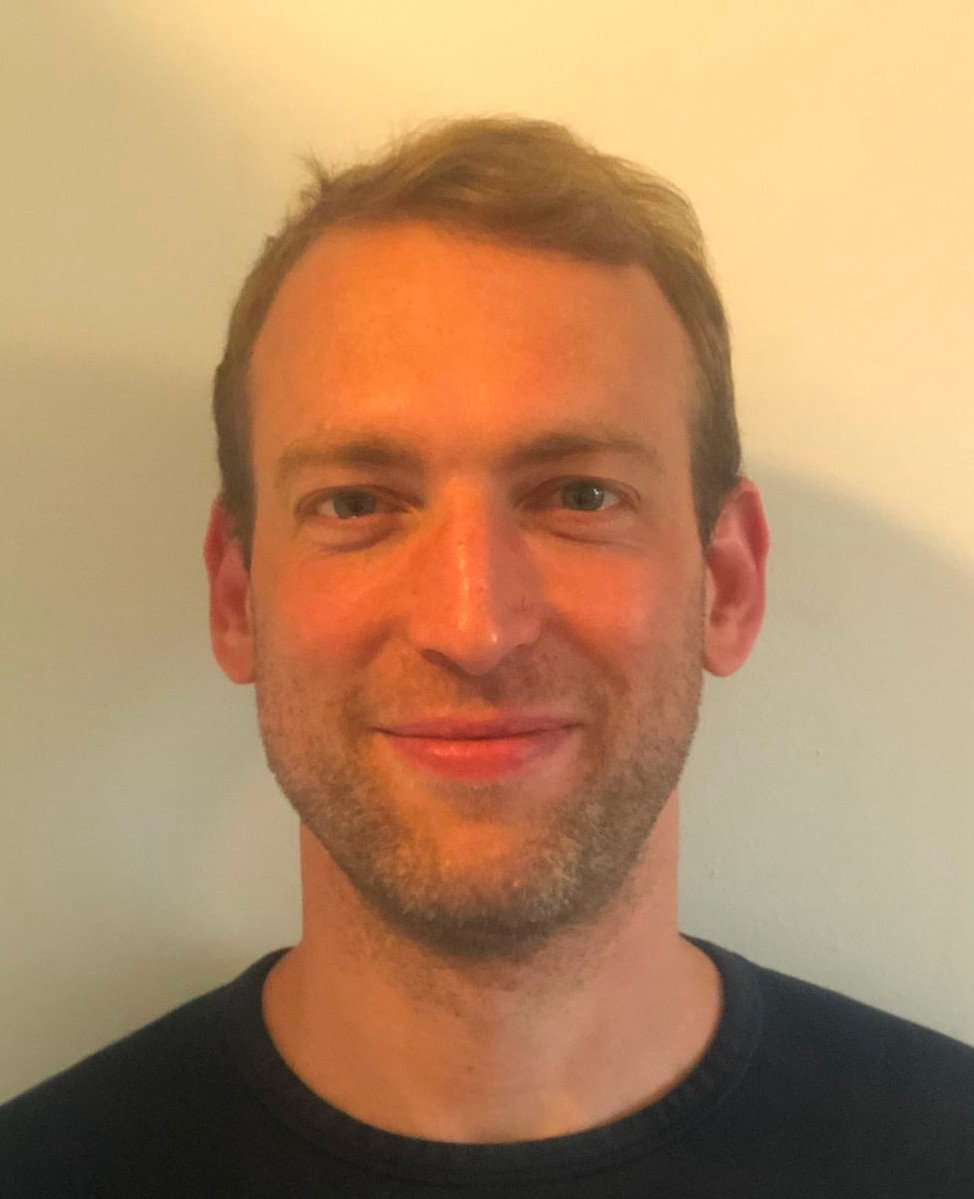
\includegraphics[height=3cm]{iser.jpg}\\
			markus.iser@kit.edu\\
			
		\end{column}
		\begin{column}{0.49\textwidth}
			\centering 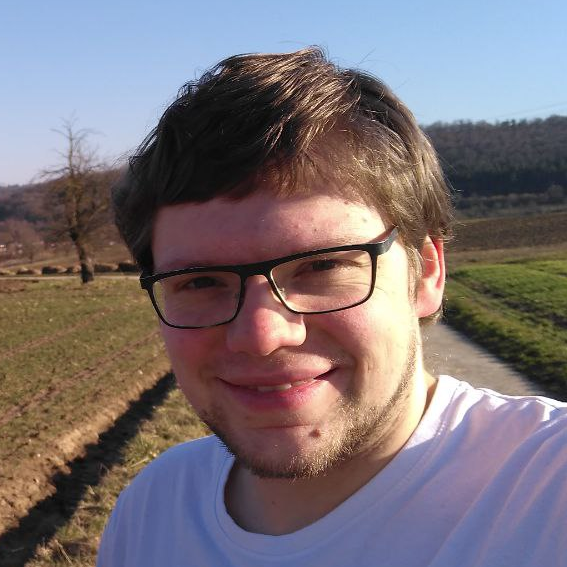
\includegraphics[height=3cm]{schreiber.png}\\
			dominik.schreiber@kit.edu
		\end{column}
	\end{columns}
\end{frame}

\begin{frame}{Topics: The Big Picture}
	\begin{itemize}
		\item Which \highl{innovative paradigms} for SAT solving and its extensions have emerged in the past few years?
		\item How can we exploit \highl{modern hardware} for \highl{dependable SAT solving} and its applications?
		\item How can we \highl{understand and exploit statistical properties} of solvers and problems?
	\end{itemize}
\end{frame}

\begin{frame}{SAT and its Extensions}
	\begin{exampleblock}{1. CDCL and Local Search}
		%\textcolor{gray}{2009, Audemard \& Simon, “Predicting Learnt Clauses Quality in Modern SAT Solvers“}\\
		2021, Cai et al., “Deep Cooperation of CDCL and local search for SAT”\\
		2022, Cai et al., “Better decision heuristics in CDCL through local search and target phases”\\
	\end{exampleblock}
	\begin{exampleblock}{2. MaxSAT}
		2016, Saikko et al., “LMHS: A SAT-IP Hybrid MaxSAT Solver”\\
		2023, Ihalainen et al., “Unifying Core-Guided and Implicit Hitting Set Based Optimization”		
	\end{exampleblock}
	\begin{exampleblock}{3. Pseudo-Boolean Reasoning}
		2020, Gocht et al., “VeriPB: The easy way to make your combinatorial search algorithm trustworthy”\\
		2024, Nieuwenhuis et al., “Speeding-up Pseudo-Boolean Propagation”
	\end{exampleblock}
\end{frame}

\iffalse
\begin{frame}{Preprocessing beyond Resolution}
	\begin{exampleblock}{4. Extended Resolution}
		2010, Audemard et al., “A Restriction of Extended Resolution for Clause Learning SAT Solvers”\\
		2023, Haberlandt et al., “Effective Auxiliary Variables via Structured Reencoding”
	\end{exampleblock}
	\begin{exampleblock}{5. Propagation Redundancy}
		2023, Reeves et al., “Preprocessing of Propagation Redundant Clauses”\\
		2023, Gao, “Kissat MAB prop in SAT Competition 2023”
	\end{exampleblock}
\end{frame}
\fi

\begin{frame}{Dependable Solving on Modern Hardware}
	\begin{exampleblock}{4. Proofs in Parallel \& Distributed SAT}
		2016, Heule et al., “Solving and verifying the boolean pythagorean triples problem via cube-and-conquer”\\
		2023, Michaelson et al., “Unsatisfiability Proofs for Distributed Solvers”\\
		2024, Schreiber, “Trusted Scalable SAT Solving with on-the-fly LRAT Checking”
	\end{exampleblock}
	\begin{exampleblock}{5. Trusted GPU-accelerated SAT Solving}
		2021, Osama et al., “SAT Solving with GPU Accelerated Inprocessing”\\
		2023, Osama et al., “Certified SAT solving with GPU accelerated inprocessing”
		%2021, Prevot et al., “Leveraging GPUs for Effective Clause Sharing in Parallel SAT Solving”
	\end{exampleblock}
\end{frame}

\begin{frame}{Data Science and Applications}
	\begin{exampleblock}{6. Applied Data Science}
		2018, Elffers et al., “Seeking Practical CDCL Insights from Theoretical SAT Benchmarks”\\
		2022, Bach et al., “A Comprehensive Study of k-Portfolios of Recent SAT Solvers”
	\end{exampleblock}
	\begin{exampleblock}{7. Future Application: Quantum Circuit Layout}
		2024, Shaik et al., “Optimal Layout Synthesis for Deep Quantum Circuits on NISQ Processors with 100+ Qubits”\\
		2024, Yang et al., “Quantum Circuit Mapping Based on Incremental and Parallel SAT Solving”
	\end{exampleblock}
	\begin{exampleblock}{8. Future Applications: XAI}
		2024, Iser, “Automated Explanation Selection for Scientific Discovery”
	\end{exampleblock}
\end{frame}





\end{document}
